\part{Common features of OpenSSH backdoors}
\section{Common features}

\begin{frame}
	\partpage
\end{frame}

%%%%%%%%%%%%%%%%%%%%%%%%%%%%%%%%%%%%%%%%%%%%%%%%%%%%%%%%%%%%%%%%%%%%%%%%%%%%%%%
\begin{frame}
	\frametitle{Strings and code obfuscation}
	
	Attackers need a way to obfuscate strings and code of backdoor (such as filenames or directories).
	
	\medskip
	
	\textbf{XOR cipher}: simplest method, encrypt the strings by xor the string with a key.
	
	\medskip
	
	\textbf{String stacking}: construct strings directly in the stack in order to bypass simple string searched.
	
	\centering
  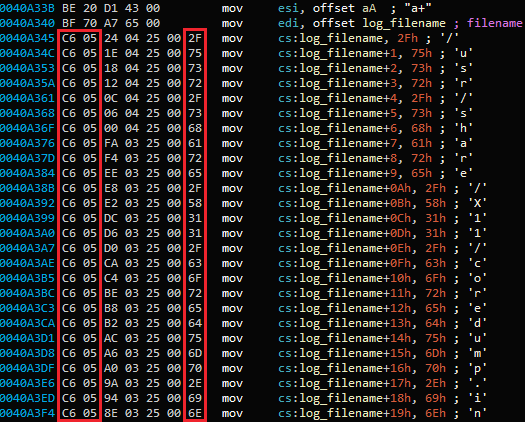
\includegraphics[width=0.4\textwidth]{images/string_stacking}
  \captionof{figure}{String stacking in a binary}

\end{frame}
%%%%%%%%%%%%%%%%%%%%%%%%%%%%%%%%%%%%%%%%%%%%%%%%%%%%%%%%%%%%%%%%%%%%%%%%%%%%%%%


%%%%%%%%%%%%%%%%%%%%%%%%%%%%%%%%%%%%%%%%%%%%%%%%%%%%%%%%%%%%%%%%%%%%%%%%%%%%%%%
\begin{frame}
	\frametitle{Credential stealing}

  Various methods to steal users credential on both sides. 

  \bigskip

	\textbf{Client}

  \smallskip

  Modify functions on client to log password on log-in such:

  \smallskip

  \textsc{userauth\_passwd}, Authenticates a session with username and password.

  \smallskip

  \textsc{ssh\_askpass}, Pass-phrase dialog.

  \bigskip

	\textbf{Server}

  \smallskip

  Modify functions on server to log password on request such:
  
  \smallskip

  \textsc{auth\_password}, Tries to authenticate the user using password.

  \smallskip

  \textsc{sshpam\_respond}, Tries to authenticate the user with PAM (Pluggable authentication modules).


\end{frame}
%%%%%%%%%%%%%%%%%%%%%%%%%%%%%%%%%%%%%%%%%%%%%%%%%%%%%%%%%%%%%%%%%%%%%%%%%%%%%%%


%%%%%%%%%%%%%%%%%%%%%%%%%%%%%%%%%%%%%%%%%%%%%%%%%%%%%%%%%%%%%%%%%%%%%%%%%%%%%%%
\begin{frame}
	\frametitle{Exfiltration methods}
	
	Once credentials are stealed, attackers need to exfiltrate them:
	
	\bigskip

	\textbf{Exfiltration by local file}
	
	\smallskip
	
	Easy method: credentials are stored inside a file in the server,
	
	hidden in filesystem (e.g.: \textsc{.so} in \textsc{/usr/bin} or \textsc{.h} in \textsc{/usr/local/include}).
	
	Problem: attackers needs to have a way back into the system.
	
	\bigskip

	\textbf{Exfiltration by C\&C server}
	
	\smallskip
	
	Complex method: send credentials over the network instead of local file.
	
	Problem: network communications are logged.
	
	Some backdoor encrypt communication with a symmetric key.
	
	\bigskip

	\textbf{Exfiltration by email}

	\smallskip
	
	In some rare cases credentials are sent by email.
	
	Problem: hardcode email address in the binary.
	
	\bigskip
	
	
\end{frame}
%%%%%%%%%%%%%%%%%%%%%%%%%%%%%%%%%%%%%%%%%%%%%%%%%%%%%%%%%%%%%%%%%%%%%%%%%%%%%%%


%%%%%%%%%%%%%%%%%%%%%%%%%%%%%%%%%%%%%%%%%%%%%%%%%%%%%%%%%%%%%%%%%%%%%%%%%%%%%%%
\begin{frame}
	\frametitle{Backdoor mode}
	
	\centering
	
  \begin{columns}
  \begin{column}{0.6\textwidth}
	Permanent Method to connect back to the compromised machine, 
	
	\medskip

	with the following features:

	\smallskip

  \textbf{Hardcoded password}, compare client password with a hardcoded password.

  \smallskip

  \textbf{Configuration and log}, change daemon configuration to permit full access and disable logging features in order to not leave traces on the system.

  \smallskip

  \textbf{Environment variables}, change environment variables such as \textsc{HISTFILE}.

  \smallskip

  \textbf{Hooked functions}, modify all functions for logging and debugging.

  \end{column}
  \begin{column}{0.35\textwidth}
      \begin{center}
      
       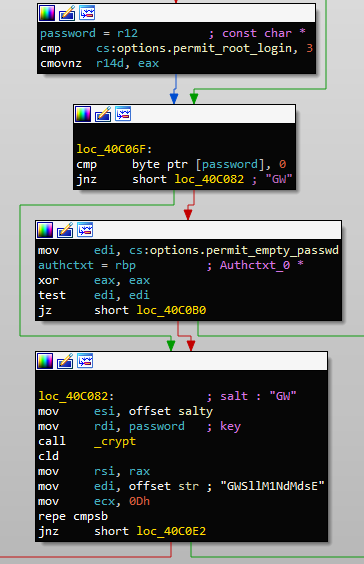
\includegraphics[width=0.9\textwidth]{images/hardcoded_password}
       \captionof{figure}{Backdoor password verification}
       \end{center}
  \end{column}
  \end{columns}

\end{frame}
%%%%%%%%%%%%%%%%%%%%%%%%%%%%%%%%%%%%%%%%%%%%%%%%%%%%%%%%%%%%%%%%%%%%%%%%%%%%%%%
